
\documentclass{iaesarticle}

%%required package. add for your convenient, but do not remove the initial
\usepackage{longtable}
\usepackage{graphicx}
\usepackage{tabularx}
\usepackage{array}
\usepackage{booktabs}
\usepackage{float}
\usepackage{longtable}
\usepackage{array}
\usepackage{longtable}
\usepackage{array}
\setlength{\headsep}{0.15in}
\usepackage{amsmath, amsfonts, amssymb, float, fancyhdr}
\usepackage[figuresright]{rotating}
\usepackage{authblk, graphicx, indentfirst, lastpage, lipsum}
\usepackage{pifont}
\renewcommand{\Authsep}{, }
\renewcommand{\Authand}{, }
\renewcommand{\Authands}{, }
\setlength{\affilsep}{0cm}
\renewcommand\Authfont{\normalsize}
\renewcommand\Affilfont{\fontsize{8}{10}\mdseries}
\makeatletter
\renewcommand{\@biblabel}[1]{[#1]\hfill}
\renewcommand\AB@authnote[1]{\textsuperscript{\normalfont\bfseries#1}}
\makeatother
\usepackage[font=normalsize]{subfig, caption}
\usepackage{epstopdf}
\usepackage[left=3cm, right=2.5cm, top=2.5cm, bottom=2.5cm, includehead, includefoot]{geometry}
\usepackage[justification=centering]{caption}
\captionsetup{labelsep=period}
\usepackage{titlesec}
\usepackage[table]{xcolor}
\titleformat{\section}
{\normalfont\normalsize\bfseries\uppercase}{\thesection}{1.7em}{}
\titleformat{\subsection}
{\normalfont\normalsize\bfseries}{\thesubsection}{.95em}{}
\titleformat{\subsubsection}
{\bfseries}{\thesubsubsection}{.2em}{}
\titlespacing*{\section}{0cm}{0.7cm}{0cm}
\usepackage{enumitem}
\usepackage[numbers]{natbib}
\usepackage{ragged2e}
\usepackage{hyperref,graphicx}
\usepackage{multirow}
\usepackage{fleqn}
\usepackage[most]{tcolorbox}
\usepackage{enumitem}
\usepackage{xcolor}

% Colores metodológicos
\definecolor{RQBlue}{HTML}{EAF3FA}
\definecolor{RQBorder}{HTML}{3F6F91}

\definecolor{IncGreen}{HTML}{EEF8F0}
\definecolor{IncBorder}{HTML}{4F8A5B}

\definecolor{ExcRed}{HTML}{FCEEEE}
\definecolor{ExcBorder}{HTML}{A95A5A}

%%leave copyright info to the editor
\CopyrightLine[]{}{\textit{This is an open access article under the \textcolor{blue}{\underline{CC BY-SA}} license.}
\vspace{.5em}}

%%author
\author[1]{\bfseries Carlos Rafael Veli Capcha}
\author[2]{\bfseries Yesenia Stefany Ramirez Medina}
\author[3]{\bfseries Axell Matias Cardenas Portocarrero}
\author[4]{\bfseries Juan Jesús Soria Quijaite}


%%author's affiliation
\affil[1]{Escuela de Ingeniería de Sistemas, Facultad de Ingeniería y Arquitectura, Universidad Peruana Unión}

%%title and shortitle (for footer)
\title{Tecnologías y sistemas inteligentes apoyados en Machine Learning para el desarrollo de habilidades de escritura grafomotoras en niños. Revisión sistemática de la Literatura.}
\shorttitle{Paper’s title should be the fewest possible words that accurately describe ... (First Author)}

%%starting
\begin{document}
\setcounter{page}{1}

%%indentation. do not change
\setlength{\parindent}{1.27cm}

%%header and footer setting. do not change
\pagestyle{fancy}
\fancyhfoffset{0cm}

%%journal info
\journalname{Bulletin of Electrical Engineering and Informatics}
\journalshortname{Bulletin of Electr Eng \& Inf}
\journalhomepage{http://beei.org}
\vol{99}
\no{1}
\months{Month}
\years{2099}
\issn{2302-9285}
\DOI{10.11591}
\pagefirst{1}
\pagelast{1x}
\id{paperID}

%%build title
\maketitle

%%border setting. do not change
\hrule
\vspace{.1em}
\hrule
\vspace{.5em}
\noindent
\parbox[t][][s]{0.315\textwidth}{%
\textbf{Article Info}
\vspace{.5em}
\hrule
\vspace{.5em}
\begin{history}
\vspace{.5em}

%%article info. editor's privilege
Received month dd, yyyy

Revised month dd, yyyy

Accepted month dd, yyyy

\vspace{.7em}
\end{history}
\vspace{.5em}
\hrule
\vspace{.5em}
\begin{keyword} 
\vspace{.5em}
%%write keyword here. separate by \sep
First keyword \sep Second keyword \sep Third keyword \sep Fourth keyword \sep Fifth keyword
\vspace{.5em}
\end{keyword}
\vspace{\fill}
}
\parbox{0.020\textwidth}{\hspace{0.5em}}
\parbox[t][][s]{0.65\textwidth}{%
\begin{abstract}
\vspace{.3em}
%% Text of abstract
An abstract is often presented separate from the article, so it must be able to stand alone. A well-prepared abstract enables the reader to identify the basic content of a document quickly and accurately, to determine its relevance to their interests, and thus to decide whether to read the document in its entirety. The abstract should be informative and completely self-explanatory, provide a clear statement of the problem, the proposed approach or solution, and point out major findings and conclusions. \textbf{The Abstract should be 100 to 200 words in length}. References should be avoided, but if essential, then cite the author(s) and year(s). Standard nomenclature should be used, and non-standard or uncommon abbreviations should be avoided, but if essential they must be defined at their first mention in the abstract itself. No literature should be cited. The keyword list provides the opportunity to add 5 to 7 keywords, used by the indexing and abstracting services, in addition to those already present in the title.
\end{abstract}
         }
\parbox[l]{\textwidth}{%
\rule{0.275\textwidth}{0.5pt} \hspace{0.5cm} \hrulefill
\\
\emph{\textbf{Corresponding Author:}}
\vspace{.5em}\\
%% correspondence info. separate by \\
Phakkharawat Sittiprapaporn\\
Neuropsychological Research Laboratory, Department of Anti-Aging and Regenerative Science\\
School of Anti-Aging and Regenerative Medicine, Mae Fah Luang University\\
Bangkok, Thailand\\
Email: wichian.sit@mfu.ac.th
}
\vspace{.5em}
\hrule
\vspace{.1em}
\hrule


%% main text

\section{Introducción}
\label{}

La escritura manuscrita constituye una habilidad compleja durante el desarrollo infantil, en la que intervienen componentes grafomotores y cognitivos que contribuyen a la calidad y fluidez del desempeño escritor. En particular, la legibilidad y la fluidez constituyen dimensiones diferenciables del desempeño de escritura y presentan relaciones distintas con las habilidades grafomotoras y otros procesos asociados \cite{Downing2023}. Asimismo, la estructura del desempeño escritor en niños que se encuentran en las primeras etapas de adquisición de la escritura puede analizarse a partir de diferentes componentes relacionados con las habilidades grafomotoras y visuomotoras \cite{Truxius2024}, \cite{Khatib2022}. Estos aspectos pueden evaluarse mediante parámetros grafomotores específicos y pruebas estandarizadas orientadas a caracterizar el desempeño de escritura infantil \cite{Sparaci2025}.

Tradicionalmente, la evaluación de la escritura infantil se ha apoyado en pruebas estandarizadas y procedimientos basados en la valoración visual del desempeño. Estos métodos permiten caracterizar la calidad de la escritura, pero pueden presentar limitaciones para registrar determinadas características dinámicas del proceso de escritura, como la velocidad, la presión y la inclinación del instrumento \cite{Asselborn2018}. La incorporación de dispositivos digitales, como tabletas y lápices electrónicos, ha permitido registrar estas variables de manera cuantitativa y ampliar la caracterización del desempeño escritor \cite{Asselborn2018}, \cite{Asselborn2020}, \cite{Philip2023}. Además, la comparación entre pruebas estandarizadas y parámetros grafomotores obtenidos mediante medios digitales ha permitido explorar diferentes dimensiones del desempeño de escritura infantil \cite{Sparaci2025}.

A partir de esta evolución, diferentes investigaciones han empleado técnicas de aprendizaje automático y aprendizaje profundo para automatizar el análisis de la escritura infantil. Estos enfoques han sido utilizados para identificar dificultades grafomotoras, detectar patrones asociados con problemas de escritura y estimar características relacionadas con el desempeño escritor. Por ejemplo, se han desarrollado modelos de aprendizaje automático para apoyar la detección de disgrafía a partir de pruebas de escritura estandarizadas \cite{Deschamps2021}, así como métodos de aprendizaje profundo orientados a la detección temprana del riesgo de disgrafía mediante aplicaciones basadas en tabletas \cite{Lomurno2023}. Asimismo, se han propuesto métodos computacionales para identificar dificultades grafomotoras mediante características derivadas del trazo \cite{Gavenciak2025}. En paralelo, se han desarrollado métodos basados en inteligencia artificial y visión computacional para identificar patrones anormales en muestras de escritura infantil \cite{Villegas-Ch2023}, evaluar habilidades de escritura mediante sistemas automatizados \cite{Inoue2025} y analizar la calidad morfológica de los trazos mediante técnicas de procesamiento de imágenes \cite{Villegas-Cubas2026}.

No obstante, la evidencia disponible presenta una considerable heterogeneidad en cuanto a las poblaciones estudiadas, las tareas de escritura, los dispositivos de captura, las características extraídas, los algoritmos empleados y los indicadores utilizados para evaluar los sistemas. Además, las investigaciones abarcan diferentes propósitos, entre ellos la detección de dificultades de escritura, la clasificación de patrones, el diagnóstico de disgrafía y la estimación cuantitativa del desempeño. Las revisiones existentes han identificado limitaciones relacionadas con tamaños muestrales reducidos, diversidad de conjuntos de datos, dependencia del idioma, diferencias metodológicas y ausencia de métricas de evaluación estandarizadas \cite{Kunhoth2024}, \cite{Fallah2025}. Esta diversidad metodológica dificulta la comparación directa entre los resultados y limita la posibilidad de establecer una visión integrada sobre las tecnologías disponibles y las características grafomotoras evaluadas.

Frente a este panorama, resulta necesario sistematizar la evidencia científica disponible para integrar los diferentes enfoques computacionales utilizados en el análisis y evaluación de la escritura infantil. Aunque se han publicado revisiones centradas en los sistemas automatizados para el diagnóstico de la disgrafía en niños \cite{Kunhoth2024} y en el uso de modelos de inteligencia artificial para la detección de esta condición \cite{Fallah2025}, estos trabajos se han concentrado principalmente en la detección o diagnóstico de dificultades de escritura. Por ello, permanece la necesidad de una síntesis que considere de manera conjunta las características de las poblaciones infantiles, las tecnologías y técnicas computacionales empleadas, los indicadores grafomotores evaluados, los métodos convencionales utilizados como referencia cuando están disponibles y los resultados de desempeño reportados por los sistemas. Una síntesis con este alcance puede contribuir a identificar tendencias, limitaciones y vacíos de conocimiento que orienten futuras investigaciones y el diseño de herramientas inteligentes para la evaluación del desempeño grafomotor infantil.

Por ello, el objetivo de la presente revisión sistemática de la literatura es analizar las tecnologías de visión computacional y las técnicas de aprendizaje automático utilizadas para evaluar habilidades grafomotoras y de escritura en población infantil. Específicamente, se busca caracterizar las poblaciones estudiadas, las tecnologías y algoritmos empleados, los métodos convencionales utilizados como referencia cuando están disponibles, los indicadores de escritura y desempeño grafomotor evaluados y los resultados de rendimiento reportados por los sistemas desarrollados.

El documento está organizado de la siguiente manera. La Sección II, Metodología, presenta el diseño metodológico de la revisión sistemática, incluyendo las preguntas de investigación, la estrategia de búsqueda, las cadenas de búsqueda empleadas en las bases de datos seleccionadas, los criterios de inclusión y exclusión, el proceso de selección de estudios conforme a PRISMA y los procedimientos de evaluación de calidad y extracción de datos. La Sección III, Resultados y Discusión, presenta los hallazgos obtenidos a partir de los estudios seleccionados y los organiza de acuerdo con las poblaciones estudiadas, las tecnologías y técnicas computacionales empleadas, los indicadores evaluados, los métodos de referencia y los resultados de desempeño. Finalmente, la Sección IV, Conclusiones, sintetiza los principales hallazgos, las limitaciones de la evidencia y las implicaciones de la revisión para futuras investigaciones.



%%metodologiaaaaaaaaaaaaaaaaaaaaaaaaaaaaaaaaaaaaaaaaaaaaaaaaaaaaaaaaaaaaaaaa
\section{Metodología}

\subsection{Diseño de la revisión sistemática}

La presente investigación se desarrolló como una revisión sistemática de la literatura (RSL), siguiendo un proceso metodológico basado en las recomendaciones de Kitchenham para la realización de revisiones sistemáticas en el ámbito de la investigación en ingeniería de software y sistemas computacionales \cite{kitchenham2007}. Asimismo, el proceso de identificación, selección y reporte de los estudios se organizó siguiendo los principios de transparencia establecidos por PRISMA.

El propósito de la revisión fue analizar las tecnologías de visión computacional y las técnicas de aprendizaje automático utilizadas para evaluar habilidades grafomotoras y de escritura en población infantil. En particular, la revisión buscó caracterizar las poblaciones estudiadas, las tecnologías y algoritmos empleados, los métodos convencionales utilizados como referencia cuando estuvieron disponibles, los indicadores de escritura y desempeño grafomotor evaluados y los resultados de desempeño reportados por los sistemas computacionales.

Para la gestión de los estudios recuperados, el proceso de revisión se realizó mediante la plataforma Parsifal, utilizada para importar los resultados de las bases de datos, identificar y marcar registros duplicados, realizar el proceso de selección, aplicar la evaluación de calidad y registrar la información correspondiente a la extracción de datos. El uso de herramientas especializadas permite centralizar y documentar diferentes actividades asociadas con la gestión de revisiones sistemáticas \cite{stefanovic2021}.

La revisión se estructuró en las siguientes etapas: definición del objetivo y preguntas de investigación, diseño de la estrategia de búsqueda, recuperación de estudios, identificación de duplicados, selección inicial de los registros mediante criterios de inclusión y exclusión, evaluación de calidad metodológica y extracción y síntesis de la información de los estudios finalmente seleccionados \cite{kitchenham2007}.

\subsection{Objetivo y preguntas de investigación}

El objetivo de la presente revisión sistemática fue analizar las tecnologías de visión computacional y las técnicas de aprendizaje automático utilizadas para evaluar habilidades grafomotoras y de escritura en población infantil. De manera específica, se buscó caracterizar las poblaciones estudiadas, las tecnologías y algoritmos empleados, los métodos convencionales utilizados como referencia cuando estuvieron disponibles, los indicadores de escritura y desempeño grafomotor evaluados y los resultados de rendimiento reportados por los sistemas.

A partir de este objetivo se formuló la siguiente pregunta principal de investigación:

\begin{center}
\fcolorbox{black!35}{blue!5}{
\begin{minipage}{0.92\textwidth}
\centering
\textbf{Pregunta principal de investigación}

\vspace{0.2cm}

\textit{¿Qué tecnologías de visión computacional y técnicas de Machine Learning han sido utilizadas para evaluar habilidades grafomotoras y de escritura en población infantil, y qué características, métodos de referencia, indicadores y resultados de desempeño han sido reportados en la literatura científica?}
\end{minipage}
}
\end{center}

\vspace{0.4cm}

Para responder de manera estructurada a la pregunta principal, se definieron cinco preguntas de investigación específicas, cada una orientada a una dimensión particular del análisis.

\begin{table}[H]
\centering
\caption{Preguntas de investigación de la revisión sistemática.}
\label{tab:preguntas-investigacion}
\renewcommand{\arraystretch}{1.35}
\small

\begin{tabularx}{\textwidth}{
    >{\centering\arraybackslash}p{1.5cm}
    >{\raggedright\arraybackslash}X
    >{\raggedright\arraybackslash}p{4.2cm}
}
\hline
\rowcolor{blue!10}
\textbf{Código} &
\textbf{Pregunta de investigación} &
\textbf{Aspecto analizado} \\
\hline

\textbf{RQ1} &
¿Qué características presentan las poblaciones infantiles estudiadas en investigaciones que utilizan visión computacional y Machine Learning para evaluar habilidades grafomotoras y de escritura? &
Población, tamaño de muestra, edad, grado escolar y condición de los participantes. \\
\hline

\textbf{RQ2} &
¿Qué técnicas y tecnologías de visión computacional y Machine Learning se han utilizado para evaluar habilidades grafomotoras y de escritura infantil? &
Dispositivos de captura, visión computacional, procesamiento de imágenes, Machine Learning y Deep Learning. \\
\hline

\textbf{RQ3} &
¿Qué métodos o instrumentos convencionales se han utilizado como referencia para evaluar las habilidades grafomotoras y de escritura infantil? &
Diagnóstico, evaluación clínica, docente o experta, pruebas estandarizadas y \textit{ground truth}. \\
\hline

\textbf{RQ4} &
¿Qué características e indicadores de la escritura y del desempeño grafomotor son evaluados mediante visión computacional y Machine Learning? &
Calidad de escritura, características del trazo, fluidez, legibilidad, precisión y velocidad. \\
\hline

\textbf{RQ5} &
¿Qué resultados de desempeño han obtenido los sistemas de visión computacional y Machine Learning utilizados para la evaluación de habilidades grafomotoras y de escritura infantil? &
Métricas de evaluación y resultados de rendimiento de los sistemas y modelos. \\
\hline

\end{tabularx}
\end{table}
Las preguntas de investigación fueron diseñadas de manera que cada una cubriera una dimensión específica de la evidencia necesaria para responder la pregunta principal. La RQ1 permitió caracterizar las poblaciones analizadas; la RQ2 permitió identificar las tecnologías y técnicas computacionales utilizadas; la RQ3 permitió determinar los métodos convencionales empleados como referencia; la RQ4 permitió identificar los indicadores de escritura y desempeño grafomotor evaluados; y la RQ5 permitió analizar las métricas y resultados de rendimiento reportados por los sistemas.

La definición de estas preguntas permitió establecer una correspondencia directa entre los objetivos de la revisión, la estrategia de búsqueda, los criterios de selección y las variables utilizadas posteriormente durante la extracción de datos.

Las preguntas fueron definidas considerando como población de interés a los niños en etapa de desarrollo de la escritura y de las habilidades grafomotoras, sin establecer un rango de edad artificialmente restrictivo.
\subsection{Estrategia de búsqueda}

La estrategia de búsqueda se diseñó a partir de los componentes conceptuales definidos para la revisión. Se consideraron términos relacionados con la población infantil, las tecnologías de inteligencia artificial y visión computacional, la escritura y los métodos de evaluación y referencia. La definición de los términos de búsqueda y su organización conceptual constituye una etapa fundamental para desarrollar una búsqueda sistemática reproducible \cite{rethlefsen2021}.

La estructura conceptual de la estrategia de búsqueda se organizó mediante los componentes PICOC. Los términos utilizados en cada componente se presentan en la Tabla~\ref{tab:picoc}.
\begin{table}[H]
\centering
\caption{Componentes PICOC y términos utilizados en la estrategia de búsqueda.}
\label{tab:picoc}

\renewcommand{\arraystretch}{1.35}
\setlength{\tabcolsep}{6pt}

\begin{tabularx}{\textwidth}{
    >{\centering\arraybackslash}m{1.8cm}
    >{\centering\arraybackslash}m{3.2cm}
    >{\raggedright\arraybackslash}X
}
\toprule

\textbf{Componente} &
\textbf{Elemento PICOC} &
\textbf{Términos utilizados} \\

\midrule

\textbf{P} &
\textbf{Population} &
\textit{child}, \textit{children}, \textit{school children},
\textit{school-age children}, \textit{pediatric},
\textit{schoolchild}, \textit{schoolchildren} \\

\addlinespace[2mm]

\textbf{I} &
\textbf{Intervention} &
\textit{machine learning}, \textit{deep learning},
\textit{artificial intelligence}, \textit{computer vision},
\textit{neural network}, \textit{image processing},
\textit{convolutional neural network},
\textit{handwriting recognition} \\

\addlinespace[2mm]

\textbf{C} &
\textbf{Comparison} &
\textit{traditional}, \textit{manual},
\textit{conventional}, \textit{expert},
\textit{teacher}, \textit{clinician},
\textit{reference}, \textit{standard},
\textit{validation}, \textit{evaluation},
\textit{assessment} \\

\addlinespace[2mm]

\textbf{O} &
\textbf{Outcome} &
\textit{handwriting}, \textit{handwriting analysis},
\textit{writing} \\

\addlinespace[2mm]

\textbf{C} &
\textbf{Context} &
\textit{school}, \textit{education} \\

\bottomrule

\end{tabularx}
\end{table}
La búsqueda se realizó en tres bases de datos científicas:

\begin{itemize}
    \item \textbf{Scopus}
    \item \textbf{Web of Science}
    \item \textbf{ScienceDirect}
\end{itemize}

Se consideraron publicaciones correspondientes al periodo \textbf{2016--2026}, en idioma inglés, de acceso abierto y correspondientes a artículos con resultados empíricos. La búsqueda fue ejecutada durante \textbf{septiembre de 2026}.

La estrategia conceptual general fue adaptada a la sintaxis específica de cada base de datos. La adaptación de una estrategia general a las características y sintaxis propias de cada fuente bibliográfica es una práctica recomendada para favorecer la reproducibilidad de las búsquedas sistemáticas \cite{rethlefsen2021}. Las cadenas utilizadas fueron las siguientes.

\subsection{Cadenas de búsqueda por base de datos}

La estrategia conceptual general fue adaptada a la sintaxis específica de cada base de datos. 
Las cadenas de búsqueda utilizadas se presentan en la Tabla~\ref{tab:cadenas-busqueda}.

\begin{longtable}{|>{\raggedright\arraybackslash}p{0.18\textwidth}|
                  >{\raggedright\arraybackslash}p{0.72\textwidth}|}
\caption{Cadenas de búsqueda utilizadas en las bases de datos científicas.}
\label{tab:cadenas-busqueda}\\
\hline
\textbf{Base de datos} & \textbf{Cadena de búsqueda} \\ 
\hline
\endfirsthead

\hline
\textbf{Base de datos} & \textbf{Cadena de búsqueda} \\ 
\hline
\endhead

% =========================
% SCOPUS
% =========================
\textbf{Scopus} &
{\footnotesize\ttfamily
(TITLE-ABS-KEY("child" OR "children" OR "school children" OR "school-age children" OR "pediatric" OR "schoolchild" OR "schoolchildren")
\newline
AND TITLE-ABS-KEY("machine learning" OR "deep learning" OR "artificial intelligence" OR "computer vision" OR "neural network" OR "image processing" OR "convolutional neural network" OR "handwriting recognition")
\newline
AND TITLE-ABS-KEY("traditional" OR "manual" OR "conventional" OR "expert" OR "teacher" OR "clinician" OR "reference" OR "standard" OR "validation" OR "evaluation" OR "assessment")
\newline
AND TITLE-ABS-KEY("handwriting" OR "handwriting analysis" OR "writing")
\newline
AND TITLE-ABS-KEY("school" OR "education"))
}
\\
\hline

% =========================
% WEB OF SCIENCE
% =========================
\textbf{Web of Science} &
{\footnotesize\ttfamily
(((ALL=("child" OR "children" OR "school children" OR "school-age children" OR "pediatric" OR "schoolchild" OR "schoolchildren"))
\newline
AND ALL=("machine learning" OR "deep learning" OR "artificial intelligence" OR "computer vision" OR "neural network" OR "image processing" OR "convolutional neural network" OR "handwriting recognition"))
\newline
AND ALL=("traditional" OR "manual" OR "conventional" OR "expert" OR "teacher" OR "clinician" OR "reference" OR "standard" OR "validation" OR "evaluation" OR "assessment"))
\newline
AND ALL=("handwriting" OR "handwriting analysis" OR "writing"))
}
\\
\hline

% =========================
% SCIENCEDIRECT
% =========================
\textbf{ScienceDirect} &
{\footnotesize\ttfamily
("child" OR "children")
\newline
AND ("machine learning" OR "computer vision")
\newline
AND ("handwriting" OR "handwriting analysis")
\newline
AND ("assessment" OR "evaluation")
}
\\
\hline

\end{longtable}

Los criterios de elegibilidad se aplicaron durante la revisión inicial de los registros recuperados. Cada artículo fue revisado individualmente y clasificado en Parsifal como \textbf{aceptado, rechazado o duplicado}. La definición explícita de criterios de inclusión y exclusión permite establecer de manera transparente las condiciones bajo las cuales un estudio puede formar parte de una revisión sistemática \cite{TUGWELL2021A5}.

Los criterios de inclusión fueron:
\subsection{Criterios de inclusión y exclusión}

Los criterios de elegibilidad se definieron previamente con el propósito de mantener un proceso de selección sistemático y transparente. Cada registro recuperado fue revisado individualmente en Parsifal y clasificado como \textbf{aceptado, rechazado o duplicado}, de acuerdo con los criterios establecidos para la revisión \cite{kitchenham2007}.

Para facilitar su identificación durante el proceso de selección, los criterios de inclusión fueron codificados como \textbf{IC} (\textit{Inclusion Criteria}), mientras que los criterios de exclusión fueron identificados como \textbf{EC} (\textit{Exclusion Criteria}).

\begin{table}[H]
\centering
\caption{Criterios de inclusión utilizados para la selección de estudios.}
\label{tab:criterios-inclusion}
\small
\renewcommand{\arraystretch}{1.35}
\begin{tabularx}{\textwidth}{|>{\centering\arraybackslash}p{1.5cm}|X|}
\hline
\rowcolor{gray!20}
\textbf{Código} & \textbf{Criterio de inclusión} \\ \hline

\textbf{IC1} &
El estudio analiza la escritura manuscrita o habilidades relacionadas con el desempeño grafomotor. \\ \hline

\textbf{IC2} &
El estudio corresponde a un artículo científico. \\ \hline

\textbf{IC3} &
El estudio fue publicado entre 2016 y 2026. \\ \hline

\textbf{IC4} &
El estudio considera población infantil en etapa de desarrollo de la escritura o habilidades grafomotoras. \\ \hline

\textbf{IC5} &
El artículo se encuentra disponible en idioma inglés. \\ \hline

\textbf{IC6} &
El texto completo se encuentra disponible gratuitamente y puede ser consultado. \\ \hline

\textbf{IC7} &
El estudio presenta resultados empíricos. \\ \hline

\textbf{IC8} &
El estudio utiliza técnicas de Machine Learning, Deep Learning, Inteligencia Artificial, visión computacional, procesamiento de imágenes u otras técnicas computacionales relacionadas con el análisis o evaluación de la escritura. \\ \hline

\end{tabularx}
\end{table}


\begin{table}[H]
\centering
\caption{Criterios de exclusión utilizados para la selección de estudios.}
\label{tab:criterios-exclusion}
\small
\renewcommand{\arraystretch}{1.35}
\begin{tabularx}{\textwidth}{|>{\centering\arraybackslash}p{1.5cm}|X|}
\hline
\rowcolor{gray!20}
\textbf{Código} & \textbf{Criterio de exclusión} \\ \hline

\textbf{EC1} &
El estudio no presenta relación con el objetivo de la revisión. \\ \hline

\textbf{EC2} &
El documento no corresponde a un artículo científico. \\ \hline

\textbf{EC3} &
El texto completo no se encuentra disponible gratuitamente. \\ \hline

\textbf{EC4} &
El estudio no considera población infantil. \\ \hline

\textbf{EC5} &
El estudio no presenta resultados empíricos. \\ \hline

\textbf{EC6} &
El estudio no utiliza técnicas de Machine Learning, Deep Learning, Inteligencia Artificial, visión computacional o procesamiento de imágenes relacionadas con el análisis o evaluación de la escritura. \\ \hline

\end{tabularx}
\end{table}

La presencia de una condición o diagnóstico particular no constituyó por sí misma un criterio de exclusión. Por ello, se consideraron estudios realizados tanto con niños sin condiciones reportadas como con niños con disgrafía, dificultades de aprendizaje u otras condiciones, registrándose esta característica posteriormente como una variable de extracción.

De igual manera, no se estableció un rango de edad rígido como criterio de exclusión. La edad y el grado escolar de los participantes fueron registrados durante la extracción de datos con el propósito de caracterizar las poblaciones estudiadas.
La presencia de una condición o diagnóstico particular no constituyó por sí misma un criterio de exclusión. Por ello, se consideraron estudios realizados tanto con niños sin condiciones reportadas como con niños con disgrafía, dificultades de aprendizaje u otras condiciones, registrándose esta característica posteriormente como una variable de extracción.

De igual manera, no se estableció un rango de edad rígido como criterio de exclusión. La edad y el grado escolar de los participantes fueron registrados durante la extracción de datos con el propósito de caracterizar las poblaciones estudiadas.

\subsection{Proceso de identificación y selección de estudios}

Los resultados obtenidos de las tres bases de datos fueron importados a Parsifal para centralizar la gestión de la revisión. Se recuperaron inicialmente \textbf{517 registros}, distribuidos de la siguiente manera:

\begin{itemize}
    \item \textbf{Web of Science:} 357 registros.
    \item \textbf{Scopus:} 52 registros.
    \item \textbf{ScienceDirect:} 108 registros.
\end{itemize}

Una vez importados los registros, se realizó la identificación de duplicados. Se detectaron \textbf{9 registros duplicados}, los cuales fueron marcados como duplicados en Parsifal y no continuaron en el proceso de selección.

Posteriormente, los registros restantes fueron revisados individualmente considerando su título, resumen y su correspondencia con los criterios de inclusión y exclusión definidos. En esta etapa se clasificaron los registros como aceptados o rechazados y, cuando un estudio fue rechazado, se registró el motivo correspondiente en Parsifal. Este procedimiento permitió documentar las decisiones adoptadas durante la selección de los estudios.

Como resultado de esta etapa, se rechazaron \textbf{465 registros}, mientras que \textbf{43 artículos fueron aceptados} para continuar con la siguiente fase de evaluación.

El flujo de selección fue:

\begin{center}
    \textbf{517 registros identificados}
    $\rightarrow$
    \textbf{9 duplicados}
    $\rightarrow$
    \textbf{508 registros evaluados}
    $\rightarrow$
    \textbf{465 rechazados}
    $\rightarrow$
    \textbf{43 aceptados}
\end{center}

El proceso de identificación, cribado, elegibilidad e inclusión de los estudios se reportó mediante un flujo basado en PRISMA 2020.

\begin{figure}[H]
    \centering
    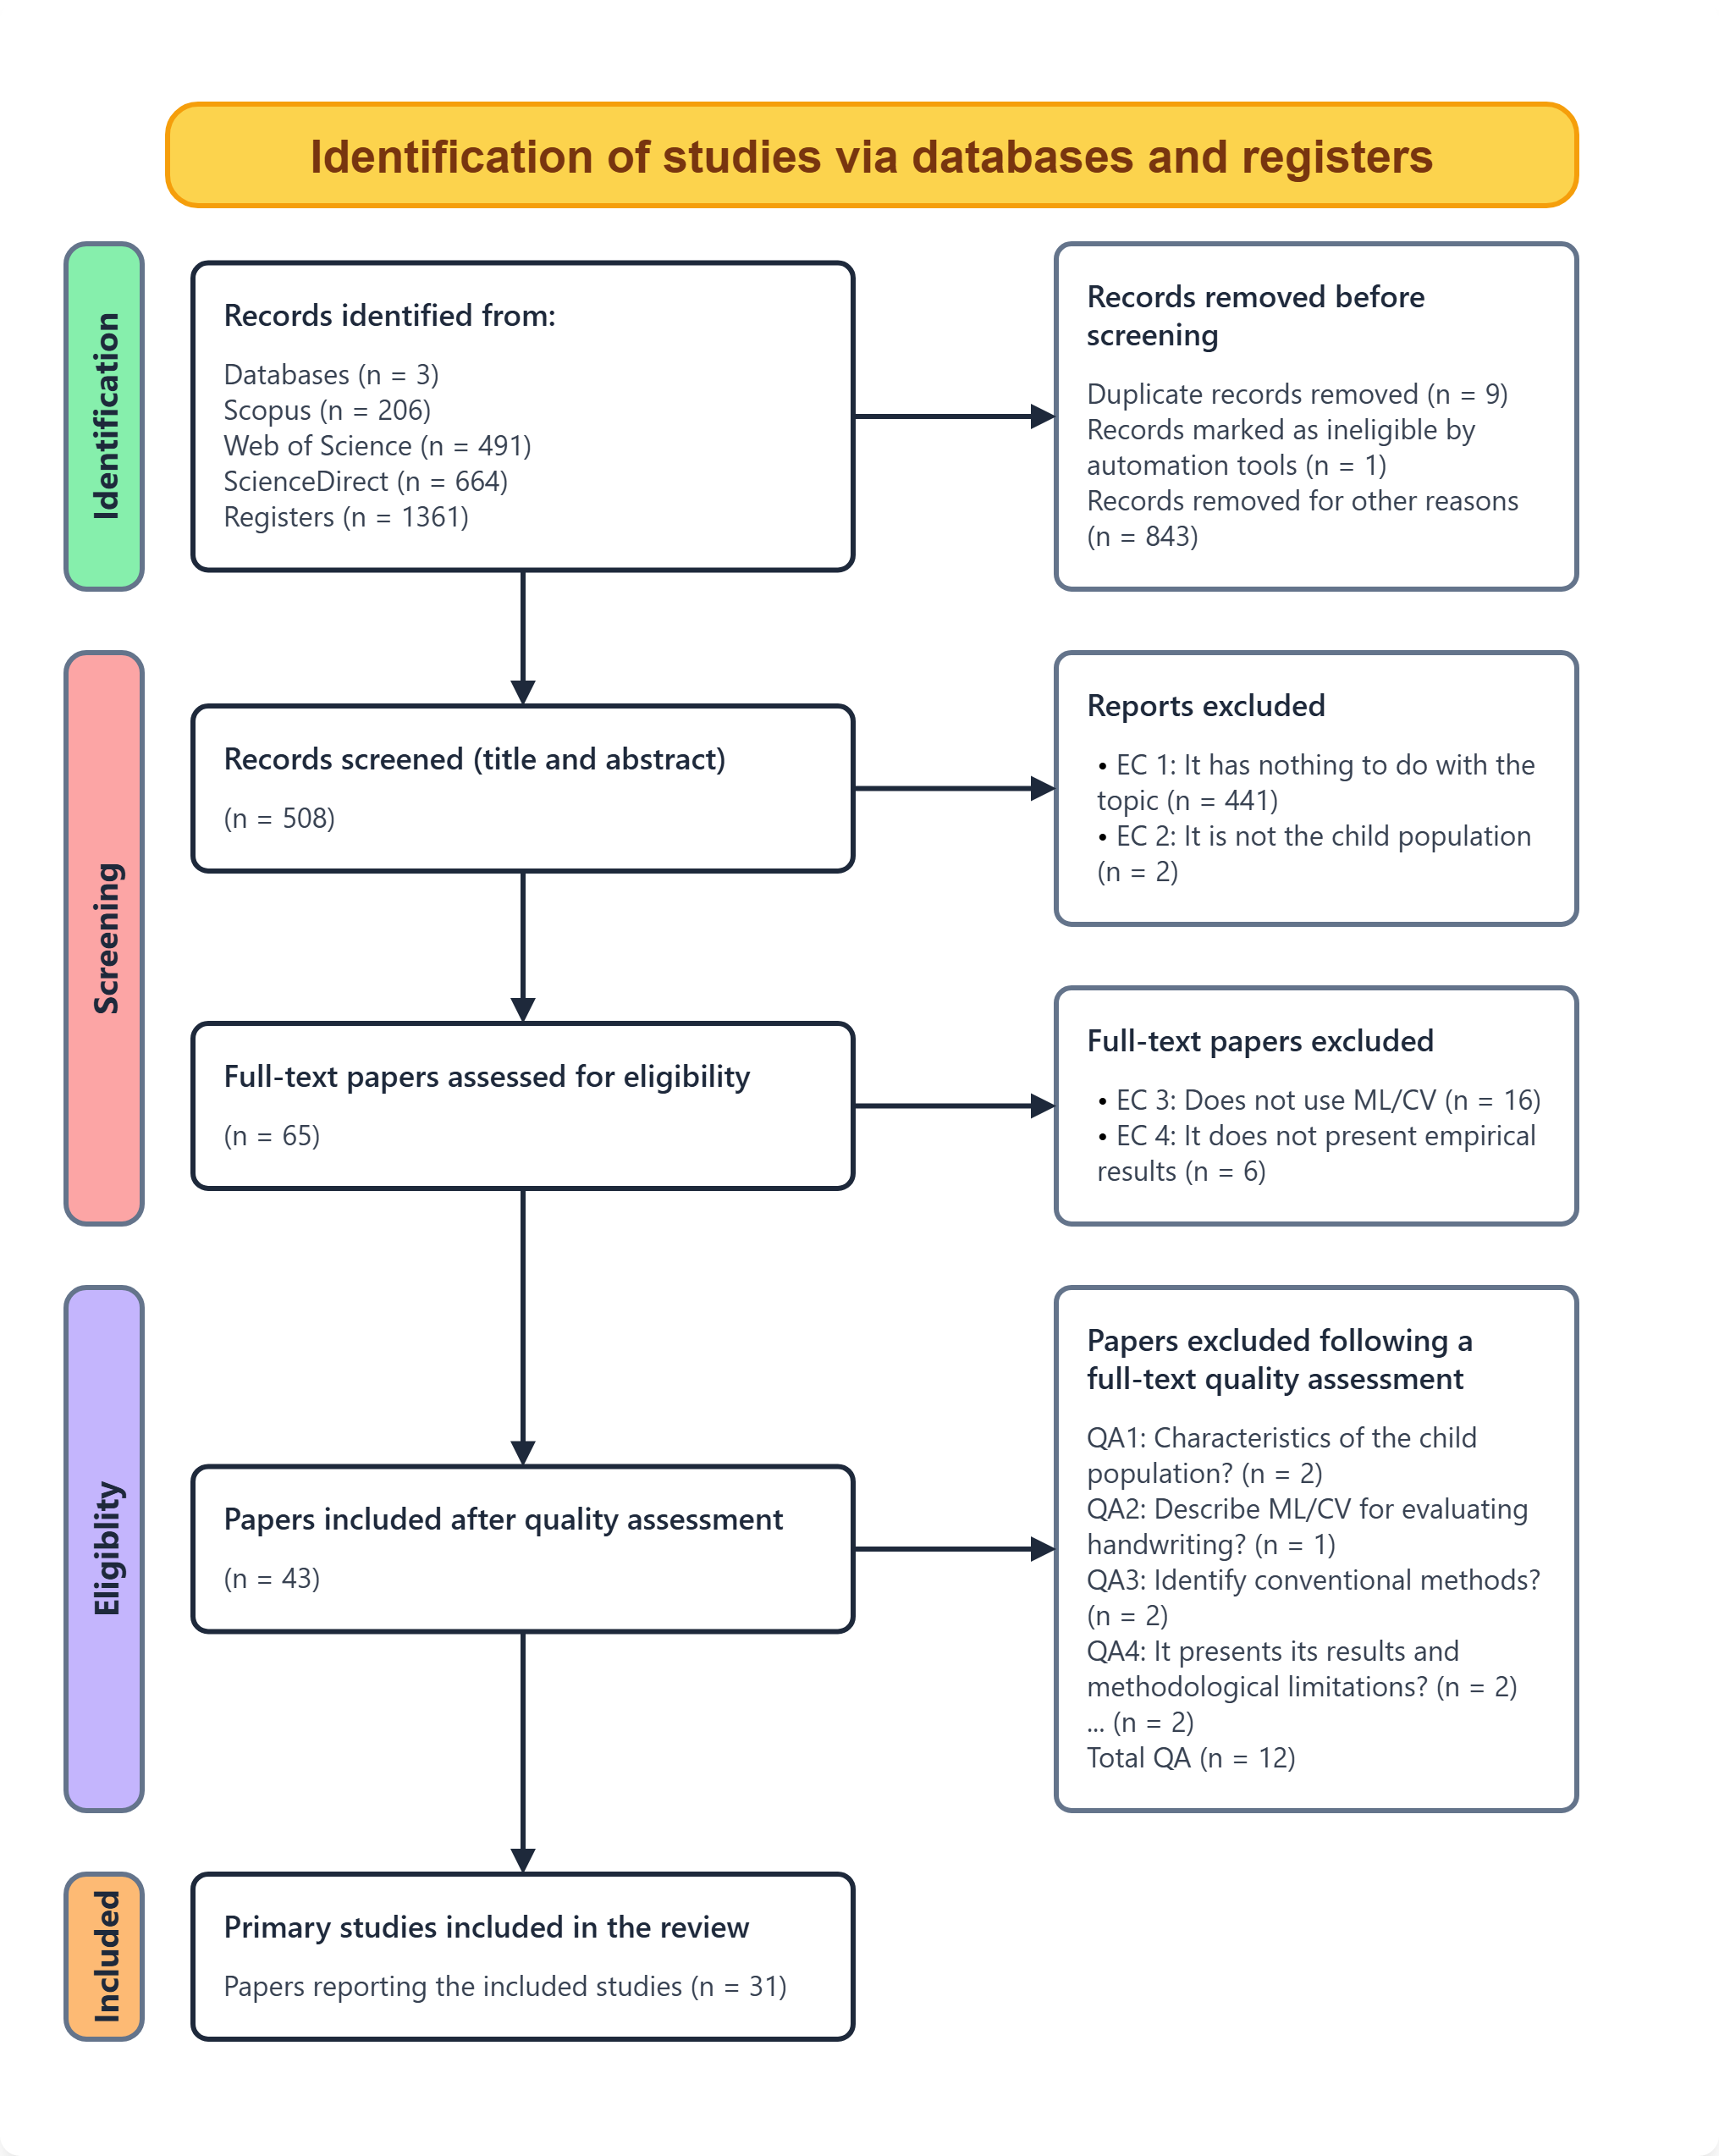
\includegraphics[width=0.90\textwidth]{images/prisma-diagram.png}
    \caption{Diagrama de flujo PRISMA del proceso de identificación y selección de estudios.}
    \label{fig:prisma}
\end{figure}

La Figura~\ref{fig:prisma} presenta el proceso de identificación, selección y evaluación de los registros recuperados. El diagrama contempla los 517 registros identificados, los 9 registros duplicados, los 465 registros excluidos durante la selección inicial y los 43 artículos que continuaron a la evaluación de calidad.

\subsection{Evaluación de calidad metodológica}

Los \textbf{43 artículos aceptados en la etapa inicial} fueron sometidos a una evaluación de calidad metodológica antes de formar parte de la muestra definitiva de la revisión. La evaluación de la calidad de los estudios primarios constituye una actividad relevante dentro de las revisiones sistemáticas, debido a que permite valorar la solidez y utilidad de la evidencia disponible \cite{kitchenham2010,kitchenham2013}.

La evaluación se realizó mediante un instrumento compuesto por \textbf{10 preguntas}, orientadas a valorar la claridad del objetivo, las características de la población, el procedimiento de adquisición de las muestras de escritura, las técnicas computacionales, los indicadores evaluados, el procedimiento de evaluación, los métodos de referencia, los resultados, la validación y las métricas de desempeño. La utilización de criterios explícitos permite establecer de forma sistemática cómo se valoró la calidad metodológica de los estudios incluidos \cite{yang2021}.

Las preguntas utilizadas fueron:
\begin{longtable}{|>{\centering\arraybackslash}m{0.07\textwidth}|m{0.84\textwidth}|}

\caption{Preguntas utilizadas para la evaluación de calidad metodológica.}
\label{tab:calidad}\\

\hline
\textbf{N.º} & \textbf{Pregunta de evaluación de calidad} \\ 
\hline
\endfirsthead

\multicolumn{2}{c}%
{{\tablename\ \thetable{} -- continuación}} \\

\hline
\textbf{N.º} & \textbf{Pregunta de evaluación de calidad} \\ 
\hline
\endhead

\hline
\multicolumn{2}{r}{Continúa en la siguiente página} \\
\endfoot

\hline
\endlastfoot

1 &
¿El estudio define claramente el objetivo relacionado con la evaluación o análisis de la escritura y/o habilidades grafomotoras infantiles? \\
\hline

2 &
¿El estudio describe claramente las características de la población infantil estudiada, incluyendo tamaño de muestra, edad, grado escolar y condición o diagnóstico cuando corresponde? \\
\hline

3 &
¿El estudio describe claramente el procedimiento utilizado para obtener las muestras de escritura, incluyendo la tarea de escritura y el dispositivo o medio de captura? \\
\hline

4 &
¿El estudio describe suficientemente las técnicas de visión computacional, procesamiento de imágenes y/o técnicas de Machine Learning utilizadas para analizar o evaluar la escritura? \\
\hline

5 &
¿El estudio describe claramente los indicadores o características de la escritura y/o desempeño grafomotor evaluados? \\
\hline

6 &
¿El estudio describe claramente el procedimiento utilizado para analizar, clasificar, evaluar o predecir el desempeño de escritura mediante el sistema computacional? \\
\hline

7 &
¿El estudio describe o identifica adecuadamente el método, instrumento, criterio convencional o referencia utilizada para evaluar el desempeño de escritura, cuando corresponde? \\
\hline

8 &
¿El estudio presenta claramente sus principales resultados y reconoce las limitaciones metodológicas o condiciones que pueden afectar la interpretación o generalización de sus hallazgos? \\
\hline

9 &
¿El estudio emplea y describe adecuadamente un procedimiento de validación o evaluación que permita valorar la confiabilidad de los resultados obtenidos? \\
\hline

10 &
¿El estudio reporta métricas o resultados cuantitativos que permitan valorar el desempeño del sistema o modelo? \\
\hline

\end{longtable}
Cada pregunta fue valorada mediante tres categorías de respuesta:
\textbf{Sí}, \textbf{Parcialmente} y \textbf{No}. A cada categoría se le
asignó una puntuación de \textbf{1}, \textbf{0.5} y \textbf{0} puntos,
respectivamente.

La puntuación máxima posible fue de \textbf{10 puntos}. Como criterio de
aceptación se estableció un puntaje \textbf{superior a 7.0 puntos}. En
consecuencia, los estudios con una puntuación igual o inferior a 7.0 fueron
excluidos de la muestra final. Este umbral fue definido previamente por los
investigadores como parte del protocolo metodológico de la revisión.

De los \textbf{43 artículos evaluados}, \textbf{31 estudios} superaron el
umbral establecido y fueron incluidos en la síntesis final, mientras que
\textbf{12 estudios} fueron excluidos durante la evaluación de calidad.

\begin{table}[H]
\centering
\caption{Resultado de la evaluación de calidad metodológica.}
\label{tab:resultado_calidad}
\renewcommand{\arraystretch}{1.3}
\begin{tabular}{|c|c|c|}
\hline
\textbf{Artículos evaluados} &
\textbf{Excluidos por calidad} &
\textbf{Estudios incluidos} \\ \hline

43 & 12 & 31 \\ \hline

\end{tabular}
\end{table}

\subsection{Participación de los revisores}

El proceso de revisión fue realizado por \textbf{tres revisores}. Los tres participaron en las actividades de selección, evaluación de calidad y análisis de los estudios, aplicando los mismos criterios de inclusión, exclusión y evaluación definidos en el protocolo de la revisión.

Para mantener la consistencia del proceso, las decisiones de selección y evaluación fueron realizadas considerando los criterios metodológicos establecidos previamente. Cuando se presentaron discrepancias o dudas respecto a la clasificación o evaluación de un estudio, estas fueron discutidas entre los revisores hasta alcanzar un acuerdo sobre la decisión correspondiente.
\subsection{Extracción de datos}

Después de la selección definitiva, los 31 estudios incluidos fueron sometidos
al proceso de extracción de datos mediante Parsifal. Para cada artículo se
registró información relacionada con la población estudiada, la tecnología y
los dispositivos de captura empleados, las técnicas computacionales utilizadas,
los indicadores grafomotores evaluados, los métodos convencionales de referencia
y los resultados reportados.

La extracción se diseñó de forma estructurada con el propósito de mantener una
correspondencia entre las preguntas de investigación, la información obtenida
de los estudios primarios y la síntesis posterior de la evidencia
\cite{cruzes2011}. Las variables consideradas se presentan en la
Tabla~\ref{tab:variables_extraccion}.

\begin{longtable}{
>{\raggedright\arraybackslash}p{0.22\textwidth}
>{\raggedright\arraybackslash}p{0.27\textwidth}
>{\raggedright\arraybackslash}p{0.43\textwidth}
}

\caption{Variables utilizadas para la extracción de datos de los estudios incluidos.}
\label{tab:variables_extraccion}\\

\toprule

\textbf{Dimensión de análisis} &
\textbf{Variable de extracción} &
\textbf{Información / categorías registradas} \\

\midrule
\endfirsthead

\multicolumn{3}{c}{
{\tablename\ \thetable{} -- continuación}
} \\

\toprule

\textbf{Dimensión de análisis} &
\textbf{Variable de extracción} &
\textbf{Información / categorías registradas} \\

\midrule
\endhead

\bottomrule
\endfoot

% =========================================================
% RQ1 - POBLACIÓN
% =========================================================

\textbf{Características de la población (RQ1)}
&
Tamaño de la muestra
&
Número de niños participantes. Cuando el estudio no reportó el número de
participantes, se registró la cantidad de muestras, imágenes o registros
analizados.
\\

\addlinespace[2mm]

&
Rango de edad
&
Edad o intervalo de edades de los participantes reportado por el estudio.
\\

\addlinespace[2mm]

&
Grado escolar
&
Nivel, grado o etapa educativa de los participantes cuando fue reportado.
\\

\addlinespace[2mm]

&
Condición de la población
&
Disgrafía; dificultades de aprendizaje; saludable; otra condición; no
especificado.
\\

\midrule

% =========================================================
% RQ2 - TECNOLOGÍA Y ADQUISICIÓN
% =========================================================

\textbf{Tecnología y adquisición de datos (RQ2)}
&
Tecnología o dispositivo de captura
&
Cámara; imagen digital; video; otro dispositivo; no especificado.
\\

\addlinespace[2mm]

&
Tipo de tarea de escritura
&
Copia; dictado; escritura libre; texto; letras/palabras; dibujo/formas;
trazado; otro; no especificado.
\\

\midrule

% =========================================================
% RQ2 - TÉCNICAS COMPUTACIONALES
% =========================================================

\textbf{Técnicas computacionales (RQ2)}
&
Técnicas de visión computacional
&
Métodos de visión computacional utilizados para procesar o analizar las
muestras de escritura.
\\

\addlinespace[2mm]

&
Procesamiento de imágenes
&
Técnicas de preprocesamiento, segmentación, extracción de contornos,
normalización, binarización u otros procedimientos reportados.
\\

\addlinespace[2mm]

&
Algoritmos o modelos de Inteligencia Artificial
&
Modelos de Machine Learning, Deep Learning, redes neuronales, CNN, SVM,
Random Forest, XGBoost u otros algoritmos utilizados.
\\

\midrule

% =========================================================
% RQ3 - MÉTODOS DE REFERENCIA
% =========================================================

\textbf{Métodos de referencia (RQ3)}
&
Método tradicional de referencia
&
Nombre del instrumento, prueba, procedimiento convencional o criterio utilizado
por el estudio como referencia para evaluar la escritura.
\\

\addlinespace[2mm]

&
Tipo de evaluación convencional
&
Diagnóstico; evaluación clínica; evaluación docente; evaluación experta;
\textit{ground truth} o etiquetado humano; prueba estandarizada; otro;
no especificado.
\\

\midrule

% =========================================================
% RQ4 - INDICADORES
% =========================================================

\textbf{Indicadores evaluados (RQ4)}
&
Indicadores grafomotores
&
Calidad de escritura; características del trazo; fluidez; legibilidad;
precisión del trazo; velocidad; otros indicadores; no especificado.
\\

\midrule

% =========================================================
% RQ5 - PROCEDIMIENTO Y RESULTADOS
% =========================================================

\textbf{Evaluación y resultados (RQ5)}
&
Procedimiento de evaluación
&
Descripción del procedimiento utilizado para analizar, clasificar, estimar
o evaluar el desempeño de escritura mediante el sistema computacional.
\\

\addlinespace[2mm]

&
Contexto de aplicación
&
Aula escolar; clínica/terapia; investigación experimental; laboratorio;
otro; no especificado.
\\

\addlinespace[2mm]

&
Métricas de desempeño
&
Accuracy, precision, recall, F1-score, sensibilidad, especificidad, AUC,
MAE, RMSE u otras métricas reportadas.
\\

\addlinespace[2mm]

&
Resultados de rendimiento del modelo
&
Valores cuantitativos reportados para el desempeño del modelo o sistema.
\\

\addlinespace[2mm]

&
Principales hallazgos
&
Conclusiones y resultados relevantes relacionados con la evaluación
computacional de la escritura o las habilidades grafomotoras.
\\

\bottomrule

\end{longtable}

La existencia de un método convencional de referencia no fue utilizada como
condición obligatoria para incluir un estudio. Esta información se registró
únicamente cuando fue reportada por los autores, en concordancia con la RQ3.

De igual manera, no se estableció un rango de edad rígido como criterio de
exclusión. La edad y el grado escolar fueron considerados variables descriptivas
para caracterizar las poblaciones analizadas.

Esta estructura permitió organizar de manera homogénea la información de los
31 estudios seleccionados y establecer una correspondencia directa entre las
variables extraídas y las cinco preguntas de investigación. Asimismo, facilitó
la posterior síntesis de resultados a pesar de la heterogeneidad existente
entre poblaciones, tareas de escritura, tecnologías de captura, algoritmos,
indicadores y métricas de desempeño \cite{cruzes2011}.

Debido a la diversidad de poblaciones, tareas de escritura, dispositivos de captura, características analizadas, algoritmos y métricas utilizadas por los estudios incluidos, la evidencia se sintetizó principalmente mediante un enfoque \textbf{descriptivo y narrativo}. La literatura revisada presenta diferentes propósitos, incluyendo la detección de dificultades de escritura, la clasificación de patrones y la estimación cuantitativa del desempeño, por lo que una comparación directa de todos los resultados mediante una única métrica no resulta apropiada \cite{cruzes2011,campbell2020}.

La síntesis se organizó de acuerdo con las preguntas de investigación:

\begin{itemize}
    \item \textbf{RQ1:} se analizaron las características de las poblaciones, incluyendo tamaño muestral, edad, grado escolar y condición o diagnóstico.

    \item \textbf{RQ2:} se identificaron y agruparon las tecnologías de captura, técnicas de visión computacional, procesamiento de imágenes y algoritmos de Machine Learning y Deep Learning.

    \item \textbf{RQ3:} se caracterizaron los métodos e instrumentos convencionales utilizados como referencia cuando fueron reportados.

    \item \textbf{RQ4:} se agruparon los principales indicadores de escritura y desempeño grafomotor evaluados.

    \item \textbf{RQ5:} se analizaron las métricas y resultados de rendimiento reportados por los sistemas y modelos.
\end{itemize}

Además de la síntesis narrativa, se utilizaron estadísticas descriptivas, frecuencias y distribuciones para representar la presencia de determinadas características entre los estudios seleccionados. Estos resultados se presentan mediante tablas y gráficos en la sección de resultados para facilitar la identificación de tendencias en la literatura \cite{cruzes2011,campbell2020}.

\subsection{Consideraciones sobre validez y limitaciones de la revisión}

La revisión presenta algunas posibles fuentes de limitación relacionadas con el proceso de búsqueda y selección. En primer lugar, la búsqueda estuvo restringida a tres bases de datos: Scopus, Web of Science y ScienceDirect, por lo que podrían existir estudios relevantes publicados en otras fuentes bibliográficas. Las restricciones en las fuentes de información pueden afectar el alcance de una revisión sistemática y deben ser consideradas al interpretar sus resultados.

Asimismo, se consideraron únicamente publicaciones en inglés y artículos con texto completo disponible gratuitamente, lo que puede limitar la recuperación de evidencia publicada en otros idiomas o de estudios cuyo acceso no se encontrara disponible durante el proceso de revisión.

La diversidad metodológica observada entre los estudios también constituye una consideración importante para la interpretación de los resultados. Las investigaciones difieren en población, tareas de escritura, dispositivos de captura, características analizadas, algoritmos y métricas de evaluación. Esta heterogeneidad constituye una consideración relevante al momento de sintetizar evidencia proveniente de estudios con características metodológicas diferentes.

Finalmente, la participación de tres revisores y la resolución de discrepancias mediante discusión buscaron mantener un proceso organizado y consistente. La evaluación mediante las 10 preguntas de calidad permitió, además, establecer un umbral explícito para determinar qué estudios formarían parte de la síntesis final.

\subsection{Resumen del proceso metodológico}

En términos generales, la revisión siguió el siguiente flujo:

\begin{center}
\begin{minipage}{0.90\textwidth}
\centering
\textbf{Definición del objetivo y preguntas de investigación}
$\rightarrow$
\textbf{diseño de la estrategia de búsqueda}
$\rightarrow$
\textbf{búsqueda en Scopus, Web of Science y ScienceDirect}
$\rightarrow$
\textbf{importación de registros a Parsifal}
$\rightarrow$
\textbf{identificación de duplicados}
$\rightarrow$
\textbf{selección mediante criterios de inclusión y exclusión}
$\rightarrow$
\textbf{43 artículos aceptados}
$\rightarrow$
\textbf{evaluación de calidad mediante 10 preguntas}
$\rightarrow$
\textbf{exclusión de estudios con puntuación $\leq 7.0$}
$\rightarrow$
\textbf{31 estudios incluidos}
$\rightarrow$
\textbf{extracción de datos}
$\rightarrow$
\textbf{síntesis descriptiva y narrativa de la evidencia}.
\end{minipage}
\end{center}





%%resultadossssssssssssssssssssssssssssssssssssssssssssssssssssssssssssssss

\section{Results and Discussion}
\label{}
This section explains the results of research and at the same time is given the comprehensive discussion. Results can be presented in figures, graphs, tables and others that make the reader understand easily [14], [15]. The discussion can be made in several sub-sections.

\subsection{Sub section 1}
Equations should be placed at the center of the line and provided consecutively with equation numbers in parentheses flushed to the right margin, as in (1). The use of Microsoft Equation Editor or MathType is preferred.

\begin{equation}
E_v - E = \frac{\hbar}{2.m}(k_x^2 + k_y^2)
\end{equation}
%% make sure to add \vspace{.005em} after the end of equation
All symbols that have not been mentioned in the equation should be explained in the following text.


\subsection{Sub section 2}
Proper citation of other works should be made to avoid plagiarism. When referring to a reference item, please use the reference number as in [16] or [17] for multiple references. The use of ”Ref [18]...” should be employed for any reference citation at the beginning of sentence. For any reference with more than 3 or more authors, only the first author is to be written followed by \emph{et al.} (e.g. in [19]). Examples of reference items of different categories shown in the References section. Each item in the references section should be typed using 8 pt font size [20]–[25].

\subsubsection {Subsub section 1}
yy

\subsubsection {Subsub section 2}
zz

\section{Conclusion}
\label{}
Provide a statement that what is expected, as stated in the "INTRODUCTION" section can ultimately result in "RESULTS AND DISCUSSION" section, so there is compatibility. Moreover, the prospects for the development of research results and the application of further studies can also be added to the next (based on the results and discussion).

\section*{ACKNOWLEDGMENTS (if applicable)}
\label{}
This section should acknowledge individuals who provided personal assistance to the work but do not meet the criteria for authorship, detailing their contributions. It is imperative to obtain consent from all individuals listed in the acknowledgments.

\section*{FUNDING INFORMATION (mandatory)}
\label{}
This section should describe sources of funding agency that have supported the work. Authors should state how the research described in their article was funded, including grant numbers if applicable. Include the following (or similar) statement if there is no funding involved: Authors state no funding involved.

\section*{AUTHOR CONTRIBUTIONS STATEMENT (mandatory)}
\label{}
This journal uses the Contributor Roles Taxonomy (CRediT) to recognize individual author contributions, reduce authorship disputes, and facilitate collaboration. \textbf{The recommended number of authors is at least two, with one of them designated as the corresponding author.} The corresponding author will be responsible for all correspondence related to the paper and must ensure that the other authors are included in the communication regarding submission, revision, and publication processes. We encourage authors to include a statement in the paper that shares and accurately describes each author's contribution. \textbf{To be eligible for authorship, each individual must have contributed to at least one of the following: conceptualization, methodology, formal analysis, or investigation, as well as at least one aspect of writing (either original draft preparation or writing reviews and editing).}

\begin{table}[H]
	\centering
	\selectfont
	\begin{tabular}{lcccccccccccccc}
		\hline
		\textbf{Name of Author}\quad\quad\quad\quad\quad\quad & \cellcolor[HTML]{D8F0F8}\textbf{C} & \cellcolor[HTML]{D8F0F8}\textbf{M} & \textbf{So} & \textbf{Va} & \cellcolor[HTML]{D8F0F8}\textbf{Fo} & \cellcolor[HTML]{D8F0F8}\textbf{I} & \textbf{R} & \textbf{D} & \cellcolor[HTML]{FDE9D9}\textbf{O} & \cellcolor[HTML]{FDE9D9}\textbf{E} & \textbf{Vi} & \textbf{Su} & \textbf{P} & \textbf{Fu} \\
		\hline
		Author 1 name & \cellcolor[HTML]{D8F0F8}\checkmark & \cellcolor[HTML]{D8F0F8}\checkmark & \checkmark & \checkmark & \cellcolor[HTML]{D8F0F8}\checkmark & \cellcolor[HTML]{D8F0F8}\checkmark &  & \checkmark & \cellcolor[HTML]{FDE9D9}\checkmark & \cellcolor[HTML]{FDE9D9}\checkmark &  &  & \checkmark &  \\
		Author 2 name &  \cellcolor[HTML]{D8F0F8}& \cellcolor[HTML]{D8F0F8}\checkmark &  &  & \cellcolor[HTML]{D8F0F8} & \cellcolor[HTML]{D8F0F8}\checkmark &  & \checkmark & \cellcolor[HTML]{FDE9D9}\checkmark & \cellcolor[HTML]{FDE9D9}\checkmark & \checkmark & \checkmark &  &  \\
		Author 3 name & \cellcolor[HTML]{D8F0F8}\checkmark & \cellcolor[HTML]{D8F0F8} & \checkmark & \checkmark & \cellcolor[HTML]{D8F0F8} & \cellcolor[HTML]{D8F0F8}\checkmark &  &  & \cellcolor[HTML]{FDE9D9}\checkmark & \cellcolor[HTML]{FDE9D9} & \checkmark &  & \checkmark & \\
		... & \cellcolor[HTML]{D8F0F8} & \cellcolor[HTML]{D8F0F8} &  &  &\cellcolor[HTML]{D8F0F8} & \cellcolor[HTML]{D8F0F8} &  &  & \cellcolor[HTML]{FDE9D9} & \cellcolor[HTML]{FDE9D9} &  &  &  & \\
		Author x name & \cellcolor[HTML]{D8F0F8} & \cellcolor[HTML]{D8F0F8} &  &  & \cellcolor[HTML]{D8F0F8}\checkmark & \cellcolor[HTML]{D8F0F8} &\checkmark &  & \cellcolor[HTML]{FDE9D9} & \cellcolor[HTML]{FDE9D9}\checkmark &  & \checkmark &  & \checkmark\\
		\hline
		\multicolumn{15}{c}{
				\begin{tabular}{llllll}
				&&&&&\\
				C &: 	\textbf{C}\fontsize{8}{10}\selectfont onceptualization \quad\quad\quad\quad\quad\quad& I &: 	\textbf{I}\fontsize{8}{10}\selectfont nvestigation & Vi&: 	\textbf{Vi}\fontsize{8}{10}\selectfont sualization  \\
				M &: 	\textbf{M}\fontsize{8}{10}\selectfont ethodology & R &: 	\textbf{R}\fontsize{8}{10}\selectfont esources & Su&: 	\textbf{Su}\fontsize{8}{10}\selectfont pervision  \\
				So&: 	\textbf{So}\fontsize{8}{10}\selectfont ftware & D &:	\textbf{D}\fontsize{8}{10}\selectfont ata Curation & P &: 	\textbf{P}\fontsize{8}{10}\selectfont roject Administration  \\
				Va&: 	\textbf{Va}\fontsize{8}{10}\selectfont lidation & O &:	\fontsize{8}{10}\selectfont Writing - \fontsize{10}{12}\selectfont \textbf{O}\fontsize{8}{10}\selectfont riginal Draft & Fu&: 	\textbf{Fu}\fontsize{8}{10}\selectfont nding Acquisition \\
				Fo&: 	\textbf{Fo}\fontsize{8}{10}\selectfont rmal Analysis & E &:	\fontsize{8}{10}\selectfont Writing - Review \& \fontsize{10}{12}\selectfont\textbf{E}\fontsize{8}{10}\selectfont diting \quad\quad\quad\quad\quad\quad&  \\
			\end{tabular}
		}
	\end{tabular}
\end{table}



\newpage\noindent See the examples below:
\begin{table}[H]
	\centering
\selectfont
	\begin{tabular}{lcccccccccccccc}
		\hline
		\textbf{Name of Author} & \cellcolor[HTML]{D8F0F8}\textbf{C} & \cellcolor[HTML]{D8F0F8}\textbf{M} & \textbf{So} & \textbf{Va} & \cellcolor[HTML]{D8F0F8}\textbf{Fo} & \cellcolor[HTML]{D8F0F8}\textbf{I} & \textbf{R} & \textbf{D} & \cellcolor[HTML]{FDE9D9}\textbf{O} & \cellcolor[HTML]{FDE9D9}\textbf{E} & \textbf{Vi} & \textbf{Su} & \textbf{P} & \textbf{Fu} \\
		\hline
		Abderrahim Taouni & \cellcolor[HTML]{D8F0F8}\checkmark & \cellcolor[HTML]{D8F0F8}\checkmark & \checkmark & \checkmark & \cellcolor[HTML]{D8F0F8}\checkmark &\cellcolor[HTML]{D8F0F8} \checkmark &  & \checkmark & \cellcolor[HTML]{FDE9D9}\checkmark &\cellcolor[HTML]{FDE9D9} \checkmark &  &  & \checkmark &  \\
		Nasreen Badruddin & \cellcolor[HTML]{D8F0F8} & \cellcolor[HTML]{D8F0F8}\checkmark &  &  & \cellcolor[HTML]{D8F0F8} & \cellcolor[HTML]{D8F0F8}\checkmark &  & \checkmark &\cellcolor[HTML]{FDE9D9} \checkmark & \cellcolor[HTML]{FDE9D9}\checkmark & \checkmark & \checkmark &  &  \\
		Phakkharawat Sittiprapaporn \quad& \cellcolor[HTML]{D8F0F8}\checkmark &\cellcolor[HTML]{D8F0F8}  & \checkmark & \checkmark & \cellcolor[HTML]{D8F0F8} & \cellcolor[HTML]{D8F0F8}\checkmark &  &  & \cellcolor[HTML]{FDE9D9}\checkmark &\cellcolor[HTML]{FDE9D9}  & \checkmark &  & \checkmark & \checkmark\\
		\hline
	\end{tabular}
\end{table}

\section*{CONFLICT OF INTEREST STATEMENT (mandatory)}
\label{}
To ensure fair and objective decision-making, authors must declare any associations that pose a conflict of interest (financial, personal, or professional) in connection with manuscripts. Non-financial competing interests include a declaration of political, personal, religious, ideological, academic, and intellectual competing interests. The authors declare that they have no known competing financial interests or personal relationships that could have appeared to influence the work reported in this paper. If there are no conflicts of interest, please include the following author's statement: Authors state no conflict of interest.

\section*{INFORMED CONSENT (if applicable)}
\label{}
The protection of privacy is a legal right that must not be breached without individual informed consent. In cases where the identification of personal information is necessary for scientific reasons, authors should obtain full documentation of informed consent, including written permission from the patient prior to inclusion in the study. Incorporate the following (or a similar) statement: We have obtained informed consent from all individuals included in this study.

\section*{ETHICAL APPROVAL (if applicable)}
\label{}
When papers talk about using people or animals, authors should make it clear that the research followed all national rules and institutional policies, and it was approved by the authors' institutional review board or a similar committee. The Helsinki Declaration's tenets must guide all investigations involving human subjects. Authors must also identify the committee or review board approving the experiments and provide a statement indicating approval of the research. Incorporate the following (or a similar) statement: The research related to human use has been complied with all the relevant national regulations and institutional policies in accordance with the tenets of the Helsinki Declaration and has been approved by the authors' institutional review board or equivalent committee; or: The research related to animal use has been complied with all the relevant national regulations and institutional policies for the care and use of animals.

\section*{DATA AVAILABILITY (mandatory)}
\label{}
The data availability statement is a valuable link between a paper’s results and the supporting evidence. It is a brief statement about whether the authors of an article have made the evidence supporting their findings available, and if so, where readers may access it. Data availability statements help to promote transparency and reproducibility in research and to increase the visibility of valuable evidence produced or gathered during the course of research. As part of our commitment to supporting open research, our journal now requires all manuscripts to include a data availability statement in order to be accepted for publication. Examples:
\begin{itemize}[topsep=0.3ex, itemsep=0.3ex, parsep=0.2ex]
	\item[-] The supporting data of this study are openly available in [repository's name] at http://doi.org/[doi], reference number [reference number].
	\item[-] The data that support the findings of this study will be available in [repository's name] [URL / DOI link] following a [6 month] embargo from the date of publication to allow for the commercialization of research findings.
	\item[-] The data that support the findings of this study are available on request from the corresponding author, [initials: AB]. The data, which contain information that could compromise the privacy of research participants, are not publicly available due to certain restrictions.
	\item[-] Derived data supporting the findings of this study are available from the corresponding author [initials: AB] on request.
	\item[-] The data that support the findings of this study are available from [third party]. Restrictions apply to the availability of these data, which were used under license for this study. Data are available [from the authors / at URL] with the permission of [third party].
	\item[-] The authors confirm that the data supporting the findings of this study are available within the article [and/or its supplementary materials].
	\item[-] The data that support the findings of this study are available from the corresponding author, [initials: AB], upon reasonable request.
	\item[-] Data availability is not applicable to this paper as no new data were created or analyzed in this study.
\end{itemize}

\section*{REFERENCES}
\label{}
\footnotesize
The main references are international journals and proceedings. All references should be to the most pertinent, up-to-date sources, \textbf{and the minimum number of references} should be \textbf{25} (for original research papers) and \textbf{50} (for review papers). References are written in IEEE style. You can access a more comprehensive guide at http://ipmuonline.com/guide/refstyle.pdf. Use a tool such as EndNote, Mendeley, or Zotero for reference management and formatting; choose \textbf{IEEE style}. Please use a consistent format for references—see examples (8 pt):

\subsection*{[1] Journal/Periodicals}
\footnotesize
\begin{flushleft}
\textsl{Basic Format:\\}
\end{flushleft}
\vspace{-1.1em} 
J. K. Author, “Title of paper,” \textsl{Abbrev. Title of Journal/Periodical}, vol. x, no. x, pp. xx-xx, Abbrev. Month, year, doi: xxx.\\ 
\emph{Examples:}
\begin{enumerate} [leftmargin=*, topsep=0.3ex, itemsep=0.3ex, parsep=0.2ex]
\footnotesize
\item[$-$] M. M. Chiampi and L. L. Zilberti, “Induction of electric field in human bodies moving near MRI: An efficient BEM computational procedure,” \textsl{IEEE Transaction on Biomedical Engineering}, vol. 58, pp. 2787–2793, Oct. 2011, doi: 10.1109/TBME.2011.2158315.
\item[$-$] R. Fardel, M. Nagel, F. Nuesch, T. Lippert, and A. Wokaun, “Fabrication of organic light emitting diode pixels by laser-assisted forward transfer,” \textsl{Appl. Phys. Lett.}, vol. 91, no. 6, Aug. 2007, Art. no. 061103, doi: 10.1063/1.2759475.
\end{enumerate}


\subsection*{[2]	Conference Proceedings}
\footnotesize
\begin{flushleft}
\textsl{Basic Format:\\}
\end{flushleft}
\vspace{-1.1em} 
J. K. Author, “Title of paper,” \textsl{in Abbreviated Name of Conf.}, (location of conference is optional), year, pp. xxx–xxx, doi: xxx. \\
\emph{Examples:}
\begin{enumerate} [leftmargin=*, topsep=0.3ex, itemsep=0.3ex, parsep=0.2ex]
\footnotesize
\item[$-$] G. Veruggio, “The EURON roboethics roadmap,” in \textsl{Proc. Humanoids ’06: 6th IEEE-RAS Int. Conf. Humanoid Robots}, 2006, pp. 612–617, doi: 10.1109/ICHR.2006.321337. 
\item[$-$]	J. Zhao, G. Sun, G. H. Loh, and Y. Xie, “Energy-efficient GPU design with reconfigurable in-package graphics memory,” in \textsl{Proc. ACM/IEEE Int. Symp. Low Power Electron. Design (ISLPED)}, Jul. 2012, pp. 403–408, doi: 10.1145/2333660.2333752.
\end{enumerate}


\subsection*{[3] Book}
\footnotesize
\begin{flushleft}
\textsl{Basic Format:\\}
\end{flushleft}
\vspace{-1.1em} 
\footnotesize
J. K. Author, “Title of chapter in the book,” in \textsl{Title of His Published Book}, X. Editor, Ed., xth ed. City of Publisher, State (only U.S.), Country: Abbrev. of Publisher, year, ch. x, sec. x, pp. xxx–xxx. \\
\textsl{Examples:}
\begin{enumerate} [leftmargin=*, topsep=0.3ex, itemsep=0.3ex, parsep=0.2ex]
\footnotesize
    \item[$-$] A. Taflove, \textsl{Computational Electrodynamics: The Finite-Difference Time-Domain Method} in Computational Electrodynamics II, vol. 3, 2nd ed. Norwood, MA, USA: Artech House, 1996. 
		\item[$-$] R. L. Myer, “Parametric oscillators and nonlinear materials,” in \textsl{Nonlinear Optics}, vol. 4, P. G. Harper and B. S. Wherret, Eds., San Francisco, CA, USA: Academic, 1977, pp. 47–160.
\end{enumerate}


%% References
%%
%% Following citation commands can be used in the body text:
%% Usage of \cite is as follows:
%%   \cite{key}         ==>>  [#]
%%   \cite[chap. 2]{key} ==>> [#, chap. 2]
%%

%% References with BibTeX database:

\bibliographystyle{IEEEtran}
\bibliography{exportIntro}
%% Authors are advised to use a BibTeX database file for their reference list.
%% The provided style IEEEtran.bst formats references is generally used.

%% For references without a BibTeX database:

%%\begin{thebibliography} {99} 
%%\footnotesize
%%\itemsep 0pt 


%%The main references are international journals and proceedings. All references should be to the most pertinent, up-to-date sources and the minimum of references are 25. References are written in IEEE style. Please use a consistent format for references – see examples below:

%% \bibitem must have the following form:
%%   \bibitem{key}...
%%

%% \bibitem{1} M. Sigala, A. Beer, L. Hodgson, and A. O’Connor, \emph{Big Data for Measuring the Impact of Tourism Economic Development Programmes: A Process and Quality Criteria Framework for Using Big Data}. 2019.

 %%\end{thebibliography}

\section*{BIOGRAPHIES OF AUTHORS}
\normalsize 
In this section, authors are required to provide their professional biography, which should include their academic background, current position, research interests, and any significant contributions to the current study. Additionally, authors should include links to their professional profiles, such as ORCID iD (mandatory) and, if applicable, Google Scholar, Scopus Author ID, or Web of Science (WoS) ResearcherID. This helps establish the author’s academic identity and enhances the visibility of their research.

\noindent Required Information:
\begin{itemize}[topsep=0.3ex, itemsep=0.3ex, parsep=0.2ex]
	\item[-] Full name: Include the author's full name as it appears in official records. If preferred, authors may use the format consistent with his/her Scopus profile.
	\item[-] Email address for each author: Provide the author's professional email address to facilitate correspondence.
	\item[-] Social media account:
	\begin{itemize}[topsep=0.3ex, itemsep=0.3ex, parsep=0.2ex]
		\item[$\blacksquare$] ORCID iD: This is a mandatory. Each author must include their ORCID iD (https://orcid.org/), which helps link his/her research output to their identity.
		\item[$\blacksquare$] Google Scholar Profile: Include the link to the author's Google Scholar profile. If the author does not have a Google Scholar profile, they may create a new one and include the link.
		\item[$\blacksquare$] Scopus Author ID: If available, include the Scopus Author ID to enhance visibility on Scopus.
		\item[$\blacksquare$] Web of Science (WoS) ResearcherID: Include the Web of Science ResearcherID. If the author does not have a WoS profile, they may create a new one and include the link.
	\end{itemize}
	\item[-] Brief biography: Provide a concise overview of the author's academic background, research interests, notable publications, and contributions to the current paper. This should be no longer than 150 to 200 words (9 pt).
	\item[-] Professional achievements: If available, mention any important awards, recognition, or research projects the author has been involved in.
	\item[-] Photo Submission: Authors must submit a clear, professional headshot (3x4 cm). The photo should be of high quality, well-lit, and not blurry. Avoid using photos that are overly casual or low resolution.
\end{itemize}


\noindent Below is an example of how to format the biography section for each author:

\section*{BIOGRAPHIES OF AUTHORS}
%% make sure to add \vspace{-.7em} before \begin{biography}
\vspace{-.7em} 
\small
\begin{biography}[{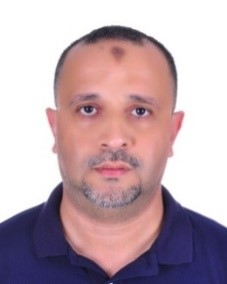
\includegraphics[width=2.5cm,height=4cm,clip,keepaspectratio]{Author1}}]
\textbf{Abderrahim Taouni} %% Affiliation and educational background.
\href{https://orcid.org/0000-0002-8070-4336}{
\includegraphics[width=0.02\textwidth]{orcid.png}} 
\href{https://scholar.google.com/citations?user=xHIMq88AAAAJ&hl=id&oi=ao}{
\includegraphics[width=0.02\textwidth]{gscholar.png}}
\href{https://www.scopus.com/authid/detail.uri?authorId=56140622700}{
\includegraphics[width=0.02\textwidth]{scopus.png}}
\href{}{
\includegraphics[width=0.02\textwidth]{wos.png}} received the Engineer degree in electrical Engineering from High Institute of Technical Education (ENSET) of Mohammedia in 1997, and the Aggregation in Electrical Engineering from the Ecole Normal Superior of Technical Education (ENSET), Rabat, in 2008. He received the Master degree in ATSII (Automatic, Signal Processing and Industrial Computing) from Faculty of Science and Technology Hassan I university Settat, MOROCCO in 2011. Currently He is Research Professor Laboratory of Industrial engineering, information processing and logistics (GITIL)-Department of Physics, Aïn Chock Science faculty- Hassan II University Casablanca, MOROCCO. His research interests include control strategies for AC machine Drives, renewable energy and batteries. He can be contacted at email: tauoni40@hotmail.com.
\end{biography}
\vspace{-.7	em}

\begin{biography}[{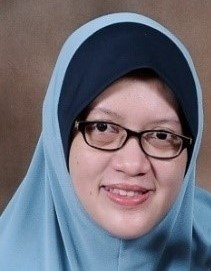
\includegraphics[width=2.5cm,height=4cm,clip,keepaspectratio]{Author22}}]
\textbf{Nasreen Badruddin} %% Affiliation and educational background.
\href{https://orcid.org/0000-0002-5666-3984}{
\includegraphics[width=0.02\textwidth]{orcid.png}} 
\href{https://scholar.google.com/citations?hl=en&user=tlGJxBwAAAAJ}{
\includegraphics[width=0.02\textwidth]{gscholar.png}}
\href{https://www.scopus.com/authid/detail.uri?authorId=18133252200}{
\includegraphics[width=0.02\textwidth]{scopus.png}}
\href{https://www.webofscience.com/wos/author/rid/AAA-4943-2021/}{
\includegraphics[width=0.02\textwidth]{wos.png}} is an Associate Professor at the Department of Electrical and Electronic Engineering, Universiti Teknologi PETRONAS, Malaysia, where she has been a faculty member since 2002. From 2015-2018, she was also the Deputy Head (Postgraduate) of the department. Nasreen graduated with a first-class honours B.Eng. degree in Electronic Engineering from RMIT University, Australia, in 2000, and an M.Sc. in Electrical \& Computer Engineering from Carnegie-Mellon University, USA in 2002. She then received the Endeavour Postgraduate Award from the Australian government in 2007 and completed her Ph.D. in Electrical \& Electronic Engineering from the University of Melbourne, Australia, in 2011. Her research interests are primarily in the area of wireless communications and networks as well as biomedical engineering, particularly in neuro-signal processing and wireless body area networks (WBAN), where she is the author/co-author of over 70 research publications. She can be contacted at email: nasreenb@ieee.org.
\end{biography}
\vspace{-.7	em}

\begin{biography}[{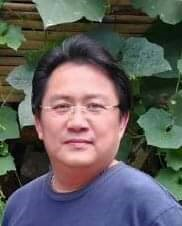
\includegraphics[width=2.5cm,height=4cm,clip,keepaspectratio]{Author3}}]
\textbf{Phakkharawat Sittiprapaporn} %% Affiliation and educational background.
\href{https://orcid.org/0000-0002-4103-9396}{
\includegraphics[width=0.02\textwidth]{orcid.png}} 
\href{https://scholar.google.com/citations?hl=en&user=vvl53FEAAAAJ}{
\includegraphics[width=0.02\textwidth]{gscholar.png}}
\href{https://www.scopus.com/authid/detail.uri?authorId=57192418814}{
\includegraphics[width=0.02\textwidth]{scopus.png}}
\href{}{
\includegraphics[width=0.02\textwidth]{wos.png}} received Bachelor of Arts (Second Class Hons.) in English from Srinakharinwirot University, Thailand, Master of Arts in Linguistics, Institute of Language and Cultural for Research and Development from Mahidol University, Thailand, and Ph.D. in Neurosciences, Neuro-Behavioural Biology Center, Institute of Science and Technology for Research and Development Mahidol University, Thailand. He was the Head of Brain Science and Engineering Innovation Research Group, Mae Fah Luang University. Currently, he is the Director of the Neuropsychological Research Laboratory, as well as a lecturer at Department of Anti-Aging and Regenerative Science School of Anti-Aging and Regenerative Medicine, Mae Fah Luang University, Bangkok, Thailand. His research interests are cognitive psychology, cognitive neurosciences, cerebral mechanisms in perception and cognition, brain mechanism of music and language perception and cognition, and neurobiology of learning and memory. He can be contacted at email: wichian.sit@mfu.ac.th.
\end{biography}

\end{document}

%%
%% End of file `iaesarticle.tex'. 